

\chapter{基于点云语义分割域适应的主动学习方法}
% \chapter{基于点云语义分割域适应的主动学习}
\thispagestyle{others}
\pagestyle{others}
\xiaosi

\section{本章引言}
本章主要介绍一种新的用于点云语义分割域适应的主动学习方法,该方法提出了一种基于源域原型指导的主动查询策略,并结合Mixing方法构建出强健的中间域数据,极大的提高了点云语义分割域适应模型的性能。接下来,本章节将首先介绍方法的研究动机和贡献,接着对每个方法子模块的原理及实现细节进行详细的介绍,最后本文将通过在主流公开数据集上取得的实验结果以及对消融实验的分析展示方法的有效性。

% \section{研究动机及贡献}
% 近年来,基于深度学习的点云语义分割方法在单一域场景下取得了显著进展,但
% 其性能高度依赖于大量标注数据。然而在实际应用中,训练的数据集与从真实环境中获取的数据集由于传感器配置、场景的不同,会产生域间隙
% 然而,在跨域场景中,目标域标注数据往往是
% 稀缺或者没有的,因此如果进行逐点人工标记则会耗费大量的人力物力,而由于域差异的存在不能直接将,所以现有方法往往面临显著的
% 域间分布差异,导致模型在目标域上的泛化能力急剧下降。而一些传统单域主动
% 学习方法\upcite{Entropy,Margin}通过选择信息量最大的样本进行标注,能够有效缓解标注成本问题。
% 然而,这些方法的样本选择策略都假定在单模态源域分布上,忽略了潜在的多模态
% 分布,而这会导致模型选择次优的目标样本并影响性能\upcite{MADA}。
% 第一,现有图像领域的主动域适应方法(如基于不确定性的边界采样[12]或基
% 于对抗学习的特征对齐[24])难以直接迁移至点云场景。点云数据具有不规则性、
% 稀疏性和几何结构敏感性,其三维空间中的局部语义关联与二维图像存在本质差
% 异。例如,图像中基于像素块或超像素的主动查询策略无法有效捕捉点云局部邻
% 域的非欧氏特征分布,导致跨域场景下的信息量评估不准确。

% 先说一些传统主动学习,然后说这些方法不适用于多模态的域适应中引用,然后说一些人开始研究新的主动域适应方法,然后举一些图像上的例子,并说明这些方法都无法直接用于点云,然后点云研究非常的少,因此探索这块领域说出问题。基于上述分析,本章的方法怎么做的相比之前的方法有何不同,提出创新性,考虑到数据的增强方式,结合mixing策略,它的优势,并且突出于mixing与AL的结合是第一次的。

% -什么方法解决了什么问题
% 介绍一下之前的方法,主动学习介绍一下,存在问题,由于域偏差的存在,不能
% 直接运用于域适应,然后主动域适应介绍一下,并没有专门的点云
% 主动域适应的策略,(介绍一些最新图像的,然后说明这些方法不适用于点云),
% 然而点云的数据结构不同于图像,由于数据模态的不同,其数据量的不同,往往
% 点云的数据量会更大,图像上的方法无法直接应用到3D点云,而在3D点云语义分
% 割中对这些方法缺乏相应的研究
% -因此本文提出了一种主动域适应策略
% -传统的主动学习方法

% 近年来,在人工智能与计算机视觉领域蓬勃发展的当下,语义分割技术作为关键的视觉任务,其重要性不言而喻。尤其是基于深度学习的语义分割方法,在图像和点云数据处理方面都取得了令人瞩目的成果。然而,这些高性能的方法往往依赖于大规模标注数据的支撑。对于三维点云而言,获取逐点标注数据是一项极为繁琐、昂贵且耗时的工作,这严重制约了相关算法的实际应用和推广。
% 为了降低标注成本并提高模型性能,主动学习方法被引入到点云语义分割任务中。现有的主动学习方法在点云语义分割领域取得了一定的进展,【】【】【】,然而,这些方法的样本选择策略都假定在单模态源域分布上,忽略了潜在的多模态分布,而这会导致模型选择次优的目标样本并影响性能\upcite{MADA}。
% 为了解决上述问题,一些学者开始致力于主动域适应的方法的研究,并在图像语义分割领域取得了一定的成果,【xxx提出】【xxx提出】然而些方法大多不能直接应用于点云语义分割。一方面,点云数据具有独特的几何结构和稀疏性,与图像数据的网格结构有本质区别;另一方面,点云的数据量庞大且无序,直接迁移图像领域的主动域适应方法无法有效捕捉点云的关键特征。
% 针对上述问题,本章提出了一种用于点云语义分割域适应的主动学习方法。该方法通过构建源域原型来指导目标点的选择,与传统主动学习方法相比,能够更有效地选择出与源域偏离程度更高的目标点,这些点往往是减小域差异的关键。此外,为了进一步提升模型的泛化能力,将主动学习与混合方法相结合,构建出包含源域和目标域选择点组成的强健中间域数据,进一步缩减域间隙。

% 本章节研究内容的主要贡献如下

% 1)提出了首个面向点云语义分割域适应的主动学习方法,超过了结合传统主动学习方法的点云语义分割域适应结果,并在极少量的标注下取得了超过最先进方法的结果。

% 2)提出了一种源域指导的目标点主动选择策略,计算目标域中候选点与源域的偏离程度,从而选择出。

% 3)将主动学习与mixing方法进行结合,构建强健的中间域数据,进一步缩减域间隙

% \section{研究动机及贡献}  
近年来,三维点云语义分割技术在自动驾驶、智能机器人等领域的应用需求日益迫切。尽管基于深度学习的全监督方法在点云语义分割上取得了显著性能,但其实际部署面临两大核心挑战:昂贵的标注成本与数据间分布差异。一方面,点云的逐点标注需耗费大量人力物力,标注单帧车载激光雷达点云需约2小时\upcite{behley2019semantickitti}。而真实场景中目标域数据因传感器配置、环境动态变化等因素,与源域存在显著分布偏移,导致模型泛化性能急剧下降\upcite{yuan2024density}。  

为缓解上述问题,现有研究主要沿两条路径展开:主动学习通过选择最具代表性的样本进行标注,以最小标注代价提升模型性能;无监督域适应则尝试在无目标域标注下对齐源域与目标域特征分布。然而,两者在跨域场景中均存在固有局限。传统主动学习方法\upcite{Entropy,Margin}的样本选择策略都假定在单模态源域分布上,忽略了潜在的多模态分布,因此选择的样本无法有效指导域间特征对齐,这会导致标注资源浪费并影响模型性能\upcite{MADA,Divide}。无监督虽无需目标域标注,但其依赖于大量的伪标签,而伪标签噪声会随迭代过程累积,限制性能提升,导致其与全监督基线仍存在很大的差异。

针对上述存在的问题,一些学者开始致力于主动域适应方法研究\upcite{AADA,CLUE,EADA能量工程},其结合主动学习和域适应方法的优势,并在图像语义分割领域取得了一定的成果,然而这些方法大多不能直接应用于点云语义分割。一方面,点云数据具有独特的几何结构和稀疏性,与图像数据的网格结构有本质区别;另一方面,点云的数据量庞大且无序,直接套用图像领域的主动域适应方法无法有效捕捉点云的关键特征。在三维点云中,Annotator\upcite{Annotator}提出了一种以体素为中心的主动学习方法,用以选择显著且具有代表性的体素,并随后对这些体素内的所有点进行标注。它第一次将主动学习运用到三维点云语义分割域适应中,并取得了超越其他传统主动学习方法的效果,然而它只考虑了点云特性依然忽略了域间差异。

% 3. **跨模态方法的不可迁移性**  
%    图像领域的主动域适应方法(如基于类原型对齐的AADA\upcite{su2020active}或对抗性查询\upcite{prabhu2021ada})难以直接迁移至点云任务。点云数据具有**非结构化、稀疏性**及**几何敏感性**等特性:  
%    - 图像超像素划分或区域提案策略无法捕捉点云局部邻域的几何关联(如曲率连续性);  
%    - 基于RGB特征的域差异度量忽略点云独有的反射强度、深度分布等模态信息;  
%    - 现有混合增强方法(如CutMix\upcite{yun2019cutmix})破坏点云空间连续性,导致语义上下文丢失\upcite{xiao2022polarmix}。  

通过上述分析,本章提出基于点云语义分割域适应的主动学习方法,核心思想是通过源域原型指导目标域上点的选择,并将标注后的目标点与源域点进行混合,组成中间域数据,实现标注效率与域对齐能力的协同优化。构建以下两个模块:1)域差异感知的主动查询:通过动态构建源域类别原型以代表源域,计算目标域中候选点与源域的偏离程度,筛选同时具备高不确定性与高域差异的目标点。这些样本能够精准暴露域间分布边界,指导模型聚焦于域偏移敏感区域。2)动态中间域构建:引入Mixing方法,随机从源域中采样一定比例的标注点与已标注的目标点云进行混合增强,生成兼具双域信息的中间域数据,该方法增强模型对域不变特征的提取能力,可以进一步缩减域间隙。
% 2. 动态中间域构建:为避免源域数据淹没稀疏标注的目标域信息,提出一种混合策略——随机采样与标注目标点等量的源域点云进行拼接,生成兼具双域统计特性的中间域数据。该策略通过隐式特征插值增强模型对域不变特征的提取能力,同时抑制源域主导的过拟合风险。  

% 本章贡献可归纳为:  

% 1)提出首个面向点云语义分割的主动域适应框架**,通过联合优化域差异感知标注与跨域混合训练,在目标域标注量仅为1\%时,mIoU超越现有UDA方法12.7\%,接近全监督基准的95\%。  

% 2)设计源域原型引导的主动查询机制**,基于类中心对齐量化目标点域偏离度,相比传统熵采样策略,在跨域任务中标注效率提升30\%(以单位标注量的mIoU增益衡量)。  

% 3)首次将主动学习与mixing方法进行结合,构建强健的中间域数据,进一步缩减域间隙  


本章节研究内容的主要贡献如下:

1)提出了一个面向点云语义分割域适应的主动学习方法,超过传统主动学习方法下的点云语义分割域适应结果,并在极少量的标注下取得了超过最先进方法的结果。

2)提出了一种源域指导的目标点主动选择策略,筛选出兼具高不确定性和高域差异性的目标点。

3)首次将主动学习与Mixing方法进行结合并运用到域适应领域,动态构建包含双域信息的中间域数据,进一步缩减域间隙。

% 方法优势与创新性:
% 与单域主动学习相比,本方法显式建模域间差异,避免标注由域偏移引起的伪不确定点;与被动域适应相比,通过主动标注关键目标域样本,构建强监督信号引导特征对齐。实验表明,该方法在复杂跨域场景(如昼夜转换、多城市迁移)中均表现出显著鲁棒性,为低标注成本下的三维场景理解提供了新的技术路径。

% \section{基于点云语义分割域适应的主动学习方法}
\section{基于点云语义分割域适应的主动学习}
\subsection{预备知识}
在点云语义分割域适应任务中,给定一个标注的源域数据\(\mathbf{S} = \{(\mathbf{X}_i^s, \mathbf{Y}_i^s)\}_{i=1}^{N^S}\),和一个目标域数据$\mathbf{T} = \{(\mathbf{X}_i^t)\}_{i=1}^ {N^T}$,其中\(N^T\)和\(N^S\)分别代表目标域和源域点云帧的数量,$\mathbf{X}_i \in \mathbb{R}^{{n_i} \times 4}$代表含有$(x,y,z,i)$三维坐标点和反射强度的一帧点云集合,并且$n_i$代表在第$i$帧点云中点的数量。 域适应的目标则是在主动学习方法的帮助下,将从标注的源域上训练好的预训练模型$G$迁移泛化到目标域数据上来,并在目标域上实现准确的点云语义分割。

在主动域适应场景中,给定一个未标注的目标域数据集$\mathbf{T}$,需要从中筛选出能够代表目标域且信息量最大的数据子集进行标注。利用新标注的目标域数据,源域训练的分割模型可逐步迭代调整以适应目标域分布,最终实现目标域上的精确语义分割。具体流程如下:首先,基于预训练模型$G$对目标域数据的预测结果,设计查询策略以计算每个未标注目标点的代表性度量得分;随后,选择最具代表性的目标点子集\(\mathbf{T}_l\)进行标注,并利用其参与分割模型$G$的调优,同时更新未标注目标数据集\(\mathbf{T}=\mathbf{T}-\mathbf{T}_l\)。该过程循环迭代直至达到预设的主动学习预算$B$。 
\subsection{方法概述}
本方法的总体框架如图\ref{fig:framework-3}所示。其算法流程主要由三个模块构成:
\ding{172}源域原型构建:通过分割模型从源点云中提取特征,并基于这些特征构建源域原型,并将作为源域的语义表征代表源域。
\ding{173}源原型引导的数据选择:计算未标记的目标点到原型的特征空间距离,得到原型相似度特征图,并根据最优-次优差异算法生成域差异分数,并将此分数与模型预测的不确定性分数结合,生成最终评分以指导标注候选目标点的选择。
\ding{174}动态混合中间域构建:使用Mixing方法,随机从源域中采样一定比例的标注点与已标注的目标点进行混合增强,构建出兼具双域信息的中间域数据,将此数据用于分割模型的微调,使得模型可以学习到更加稳定可靠的域不变特征,从而进一步缩减域间隙。

\vspace{-0.1cm}
\begin{figure}[h]
    \centering
    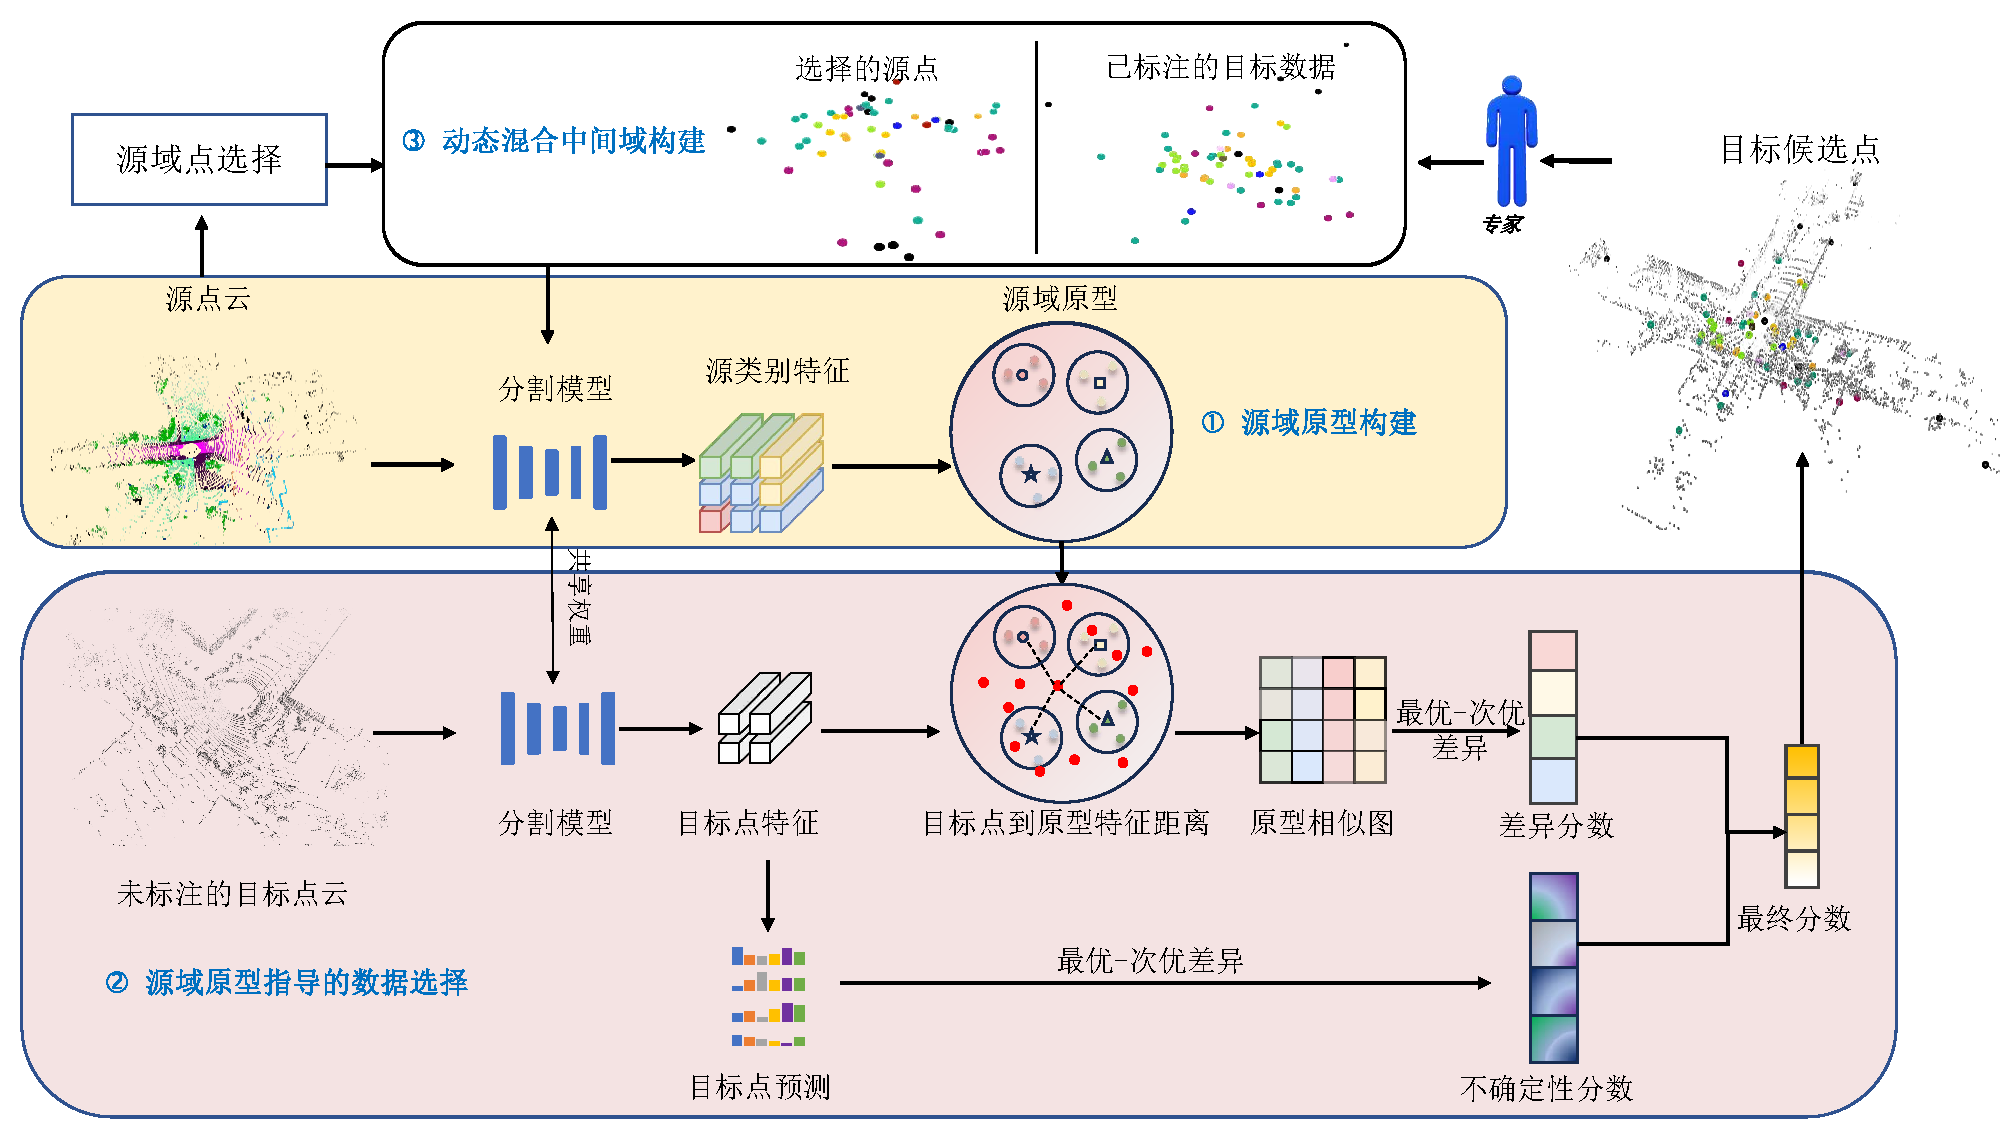
\includegraphics[width = \textwidth]{ljx/figure/3-1.pdf}
    \bicaption[\xiaosi 基于点云语义分割域适应的主动学习方法框架]{\wuhao 基于点云语义分割域适应的主动学习方法框架}{\wuhao Framework of the active learning method for domain adaptation in point cloud semantic segmentation}
    \label{fig:framework-3}
\end{figure}
\vspace{-0.35cm}
\subsection{源域原型构建}
% 当前面向点云语义分割的主动域适应方法主要利用源域预训练模型在目标域的预测结果,通过识别模型难以准确判别的"不确定性"数据来选择标注样本。然而,这类方法存在两个关键缺陷:首先,其选择过程忽略了源域与目标域之间的分布差异,导致所选样本往往集中在特定长尾类别上,使得标注数据缺乏多样性和代表性;其次,源域训练的分割模型对目标域数据的预测存在偏差,导致查询策略的可靠性降低。
% 为此,本章提出通过联合考虑预测置信度与源-目标域分布差异,实现可靠且分布均衡的数据选择。
为表征源域数据分布的结构特征,首先需要基于特征中心构建源域类别原型。具体而言,对于源域中每个类别的点云样本,利用分割模型$G$,提取其特征向量,并将同类特征向量的均值作为该类的原型表征。如图\ref{fig:3-2}所示,将标注的源域数据集$\mathbf{S}$输入到当前网络并提取特征矩阵$\mathbf{F} \in \mathbb{R}^{{N^S_P} \times d_f}$, 其中\(N^S_P\)表示源域中所有标注类别点的数量,$d_f$为特征维度,基于源数据类别信息,通过公式\eqref{eq:prototype_compute}所示计算类别原型\( \mathbf{p}^c \)。
\begin{equation}
    \label{eq:prototype_compute}
    \mathbf{p}^c = \frac{\sum_{i=1}^{N^c} \mathbf{f}_i^c}{N^c}
\end{equation}
其中,\( c \in [1, C] \)表示类别索引,\( C \)为源域类别总数;\( \mathbf{f}_i^c \)为类别\( c \)中第\( i \)个点的特征向量;\( N^c \)为类别\( c \)的样本数量,对应的公式如\eqref{eq:Nc}所示:
\begin{equation}
    \label{eq:Nc}
    % N_c = \sum_{\mathbf{f} \in \mathbf{F}} \mathbb{I}(\mathbf{f} = c),
    N^c = \sum^{N^S_P}_{i=1} \mathbb{I}(y^s_i = c)\mathbf{f}_i
\end{equation}
式中,\( y^s_i \)表示第\(i\)个源点特征\( \mathbf{f}_i \)对应的类别标签;$\mathbb{I}(y^s_i = c)$为指示函数,当$y^s_i$属于类别$c$时取值为1,否则为0。

由于点云数据集庞大,因此常规服务器设备无法一次性将所有的数据都加载到内存并进计算,而如果设计全局变量累加多次迭代的结果,可能会造成一定的精度损失和内存消耗,为了节省内存资源和保证结果的准确性,本章采用Welford增量均值算法\upcite{welford1962note}进行渐进式的原型计算,如公式\eqref{eq:incremental_equation}所示:
\begin{equation}
\label{eq:incremental_equation}
    \mathbf{p}_{b+1}^c = \mathbf{p}_b^c + \frac{\mathbf{p}_{b+1}^c - \mathbf{p}_b^c}{x_{b+1}}
\end{equation}
式中,\(\mathbf{p}_{b+1}^c\)代表在第\(b+1\)训练批次时类别\(c\)的原型结果;\(\mathbf{p}_{b}^c\)代表上一批次时类别\(c\)的原型结果;\( x_{b+1} \)则代表在第\( b+1 \)训练批次时类别\( c \)的总数量。通过该算法最终得到源域原型矩阵\( \mathbf{P} \in \mathbb{R}^{C \times {d_f}} = \{\mathbf{p}^i\}^C_{i=1} \),其中每个原型向量\(\mathbf{p}^i\)对应特征空间中源域某个类别的质心,蕴含该类别的语义特征。由于分割模型在不断微调,这些源域原型将在每一轮的主动学习阶段动态更新,根据新的模型动态的构建新的源域原型,并为后续的跨域数据选择提供指导。

\vspace{-0.1cm}
\begin{figure}[h]
    \centering
    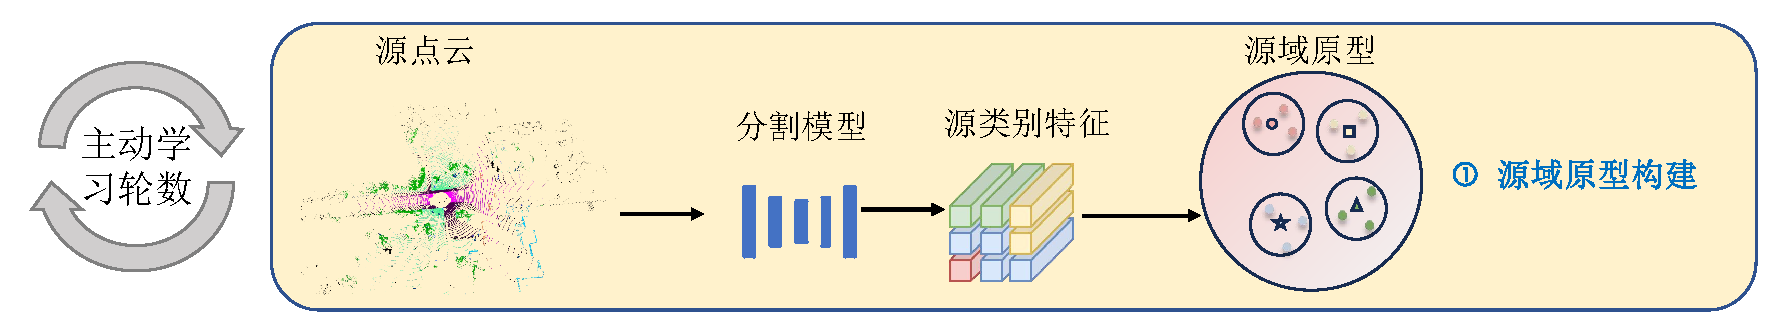
\includegraphics[width = \textwidth]{ljx/figure/3-2.pdf}
    \bicaption[\xiaosi 源域原型构建]{\wuhao 源域原型构建}{\wuhao Source prototype construction}
    \label{fig:3-2}
\end{figure}
\vspace{-0.35cm}


\subsection{源域原型指导的数据选择}
源域原型构建完成后,可将其作为基准指导目标域数据的筛选。如图\ref{fig:3-3}所示,将未标注的目标域点云输入预训练分割网络,提取其特征矩阵\( \mathbf{F}^T \in \mathbb{R}^{N^T \times d_f} \),其中\(N^T\)为目标域点数。随后逐点计算其与源域各类别原型的欧氏距离,其表达式公式如\eqref{eq:distance}所示:
\begin{equation}
    \label{eq:distance}
    \mathbf{d}_i^c = \| \mathbf{f}_i^t - \mathbf{p}^c \|
\end{equation}
式中,\( \mathbf{f}_i^t \in \mathbf{F}^T \)表示目标域第\( i \)个未标注点的特征向量;\(\mathbf{p}^c\)为源域类别\(c\)的原型向量;\( \mathbf{d}_i^c \)代表点到源域类别\(c\)的欧式距离,该距离度量反映了目标点特征与源域类别质心的空间距离,其值越小代表未标注点在特征空间中距离源域类别\( c \)的聚类中心越近;越大则表明未标注点在特征空间中距离源域类别\( c \)的聚类中心越远。因此,$\mathbf{d}_i^c$将作为一个重要的域差异计算依据,并用于后续的域差异评分的一个重要衡量指标。
% ,距离越小,表明目标点特征在源域特征空间中越接近类别\( c \)的聚类中心。

\begin{figure}[H]
    \vspace{-0.2cm}
    \centering
    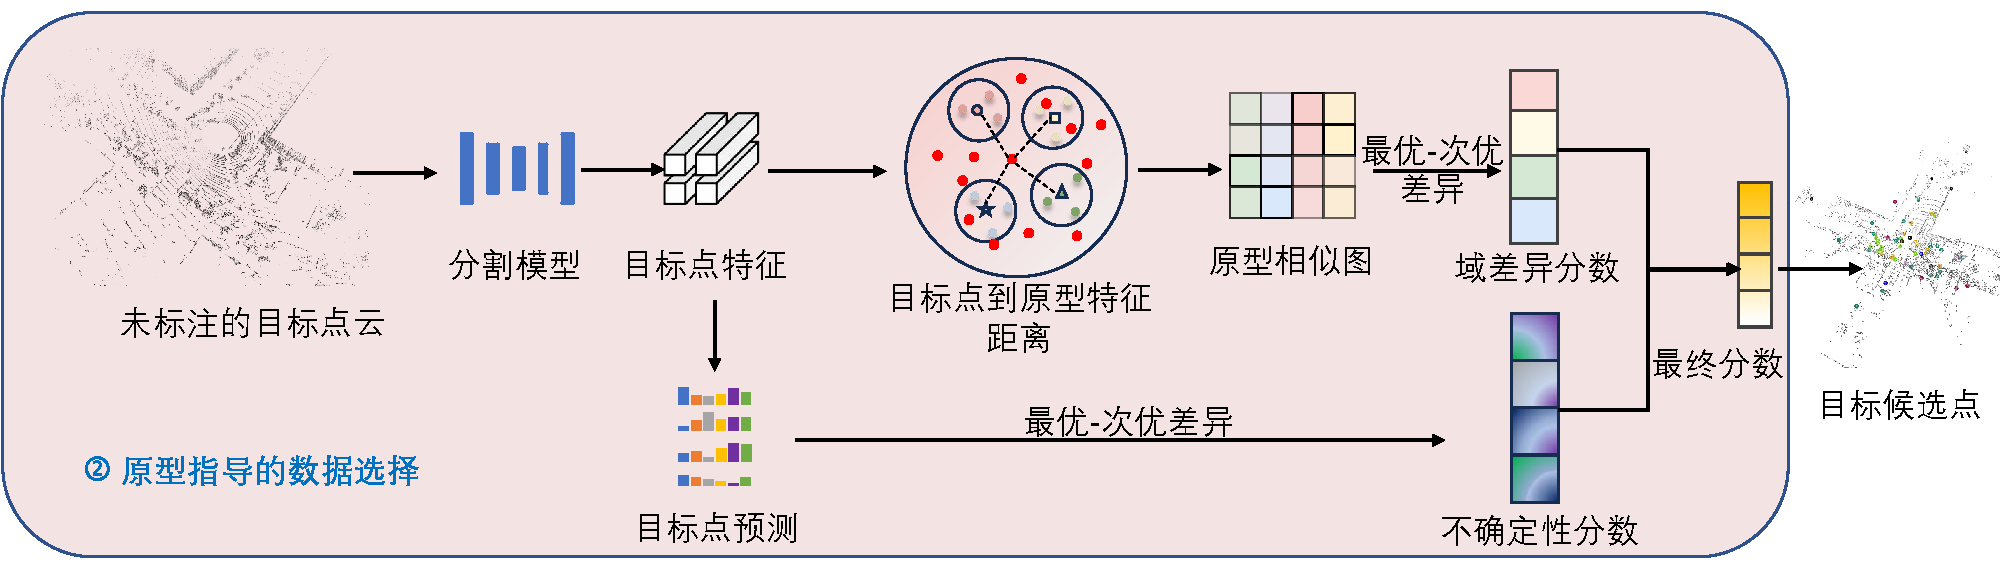
\includegraphics[width = \textwidth]{ljx/figure/3-3.pdf}
    \bicaption[\xiaosi 源域原型指导的数据选择]{\wuhao 源域原型指导的数据选择}{\wuhao Source-prototype guided data selection}
    \label{fig:3-3}
    \vspace{-0.45cm}
\end{figure}

\subsubsection{计算域差异评分}
对每个目标点\(p_i\)遍历计算与所有类别原型的特征距离,生成距离向量\( \mathbf{D}_i = [d_i^1, d_i^2, \dots, d_i^C] \)。为量化其域间分布特性,需将距离向量转换为相似性度量并进行归一化处理:

1)相似性转换:对\( \mathbf{D}_i\)逐元素取倒数,得到相似性向量\( \mathbf{D'}_i = [1/d_i^1, 1/d_i^2, \dots, 1/d_i^C] \),使得距离越近的类别相似度值越高。

2)概率归一化:通过$softmax$函数\(f(\cdot)\)将\(\mathbf{D'}_i\)映射为概率分布,如公式\eqref{eq:softmax}所示,消除量纲差异增强判别性,确保不同类别的相似值在同一尺度下比较。
% 完整公式环境示例
\begin{equation}
    \label{eq:softmax}
    f(\mathbf{D}_i') = softmax(\mathbf{D}_i') = 
    \begin{bmatrix}
    \displaystyle
    \frac{e^{d_i^{1'}}}{\sum_{c=1}^{C} e^{d_i^{c'}}}, &
    \cdots, &
    \displaystyle
    \frac{e^{d_i^{C'}}}{\sum_{c=1}^{C} e^{d_i^{c'}}}
    \end{bmatrix}
\end{equation}

最终通过最优-次优差异算法计算域差异评分\(M^i_{ds}\),公式如\eqref{eq:dis_score}所示:
\begin{equation}
    \label{eq:dis_score}
    M^i_{ds} = S_{R1}(f(\mathbf{D}_i')) - S_{R2}(f(\mathbf{D}_i'))
\end{equation}
式中,\(S_{R1}(\cdot)\)和\(S_{R2}(\cdot)\)分别表示最大概率值与次大概率值。\(M^i_{ds}\)越小,则表明目标点与两个源域类别的相似度接近,意味着其处于源域类别边界区域,这样的目标点对缓解域偏移具有更高价值。

\subsubsection{融合不确定性评分}
得到域差异评分后,为了避免选择的点都是同类别的点,融合不确定性评分进行最终筛选。通过分割头\(h(\cdot)\)获取目标点的预测概率分布\(\mathbf{p}^t_i \in \mathbb{R}^{1\times C}\),并计算其不确定性评分\( M^i_{us} \),其表达公式如公式\eqref{eq:unc_score}所示:
\begin{equation}
    \label{eq:unc_score}
    M^i_{us} = S_{R1}(\mathbf{p}_i^t) - S_{R2}(\mathbf{p}_i^t)
\end{equation}
式中,$S_{R1}$和$S_{R2}$分别代表最大和次大次大类别概率值。该评分反映模型对目标点不确定性:当\(M^i_{us}\)较小时,表明模型对该点的预测存在较高不确定性,其位于类别边界上无法区分,此类样本的标注可有效提升模型性能。
为平衡域差异特性与模型不确定性,采用加权融合策略生成最终评分,其表达式如公式\eqref{eq:fin_score}所示:
\begin{equation}
    \label{eq:fin_score}
    M^i_{final} = \alpha \times M^i_{ds} + (1 - \alpha) \times M^i_{us}
\end{equation}
其中,\(\alpha \in [0,1]\)可调节的超参数。当\(\alpha=0.5\)时,两类评分贡献均等;当目标域与源域分布差异显著时,可增大以强化域差异指导作用,因此在不同的场景下\(\alpha\)可能会有所不同。

\subsubsection{筛选候选样本}
基于最终目标评分\(M^i_{final}\),对所有目标点进行升序排列,评分越低优先级越高,选取每帧点云中排名前\(k\)的点组成候选样本点集\(\mathbf{T}_l\)提交至专家(Oracle)进行人工标注,同时更新未标注目标数据集\(\mathbf{T}=\mathbf{T}-\mathbf{T}_l\),在下一轮的主动学习中,已标注的目标点将不参与筛选,其中\(k\)与主动学习轮数\(R\)、标注总预算\(B\)以及目标点云的帧数$N^T$的关系如公式\eqref{eq:3-9}所示:
\begin{equation}
    \label{eq:3-9}
    k=\frac{B}{R \times N^T}
\end{equation}

% 此策略即考虑了目标域选择时候的域差异问题,又考虑了类别冗余的问题,即通过结合域差异评分和不确定性评分,选择兼具高域差异和高不确定性的点,可以更好的泛化和提高模型。

% 增强域适应性:优先选择域差异评分高的样本,迫使模型关注源域未充分覆盖的特征区域

% 提升标注效率:不确定性评分高的样本往往包含更多信息量,标注此类样本可快速修正模型认知盲区

\subsection{动态混合中间域构建}
最后,为了进一步增强模型的泛化能力,本算法引入了Mixing混合方法。如图\ref{fig:3-4}所示,在每一轮训练中任意一帧目标点云都会随机匹配一帧源点云,并随机从源点云中选择一定比例的源点\(\mathbf{S}_{s_i}\),将这些选择后的源点与已标注的目标点\(\mathbf{T}_{a_i}\)进行混合,组成含两域信息的中间域数据\(\mathbf{I}_i=concat(\mathbf{T_{a_i}},\mathbf{S_{s_i}})\),其中\(concat(\cdot)\)代表拼接混合。这些中间域数据可以帮助模型学习到更加可靠的域不变特征,进一步缩减域间隙\upcite{chen2021semi,wang2023ssda3d}。

\vspace{-0.1cm}
% \vspace{0.5cm}
\begin{figure}[h]
    \centering
    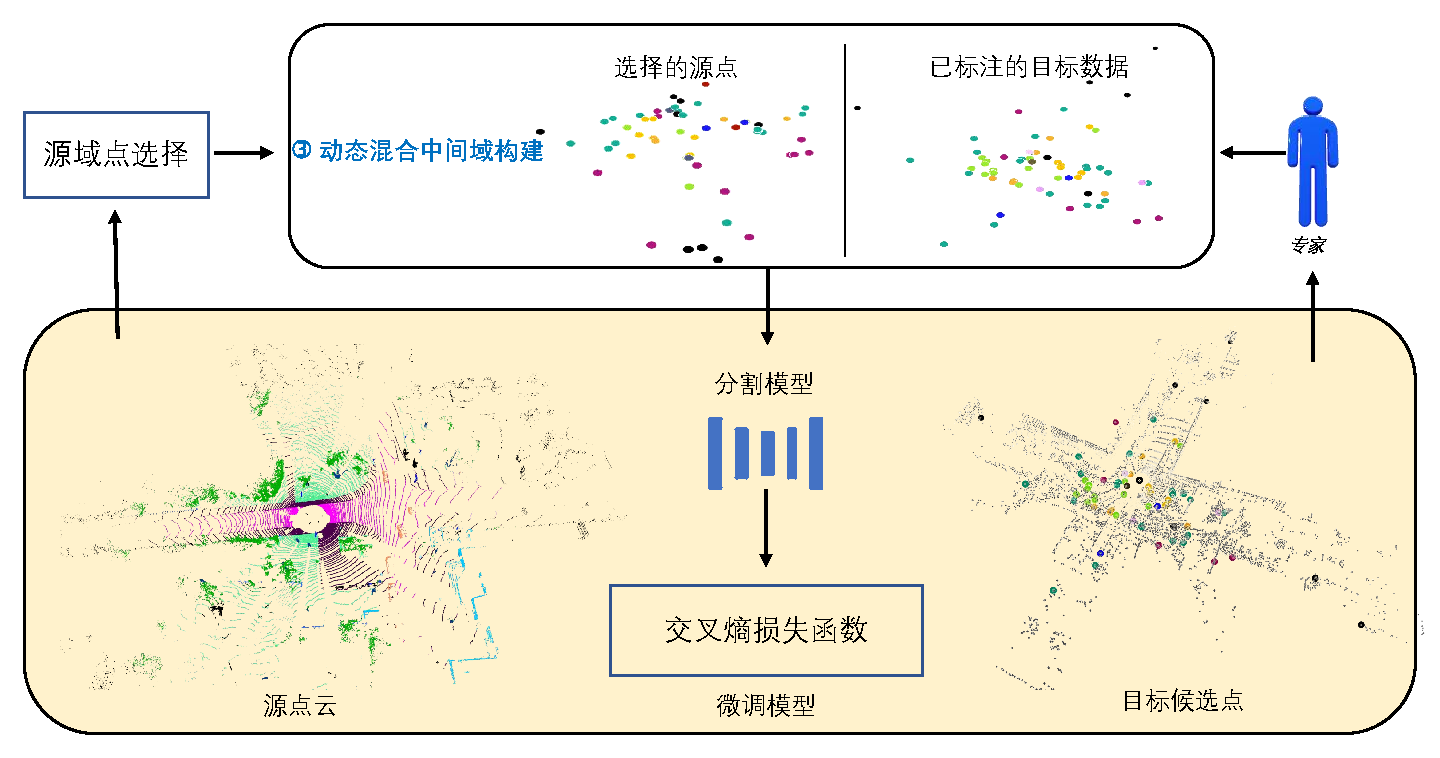
\includegraphics[width = \textwidth, scale=0.5]{ljx/figure/3-4.pdf}
    \bicaption[\xiaosi 动态混合中间域构建]{\wuhao 动态混合中间域构建}{\wuhao Dynamic mixed intermediate domain construction}
    \label{fig:3-4}
    % \vspace{-9pt}
\end{figure}
\vspace{-0.5cm}
% \subsection{损失函数}放到第4章吧
\section{实验评估}
\subsection{实验设置}
在实验中,使用MinkowskiNet\upcite{MinkowskiNet}在Annotator中的PyTorch实现版本作为目标分割网络模型,并使用随机梯度下降(SGD)\upcite{SGD}作为学习优化器,将动量设置为0.9,在第一轮的训练中使用线性预热策略,使学习率线性增加到基础学习率0.01,同时使用权重衰减系数为0.0001的余弦衰减调度器动态调整学习率,进一步稳定模型收敛,所有实验都是在单张NVIDIA RTX A6000 GPU上进行的训练。

本章方法在真实到真实及合成到真实的跨域场景下均进行了大量充分的实验,并通过详细的可视化分析验证其有效性。对于所有场景,主动学习过程共执行5次迭代,以达到预设的标注预算。
在合成到真实的跨域场景实验中,预训练模型(Source-only)和全监督模型(Target-only)阶段的批量大小设为16;在SynLiDAR$\to$SemanticKITTI实验中训练10轮,在SynLiDAR$\to$SemanticPOSS实验中训练20轮。而在域适应阶段,每一步的批量大小设为14并训练50轮。权重参数$\alpha$分别在SynLiDAR$\to$ SemanticKITTI和SynLiDAR$\to$SemanticPOSS的实验中设置为0.4和0.6。
在真实到真实的跨域场景实验中,SemanticKITTI$\to$nuScenes和nuScenes$\to$SemanticKITTI的实验配置相同,预训练模型Source-only和全监督模型Target-only阶段的每一步批量大小设为16,并训练10轮;在域适应阶段的每一步批量大小设置为10并训练50轮,权重参数$\alpha$为0.6。其中Mixing方法的随机混合比例为30,即混合后的中间域数据,源域点数是目标域点数的30倍。
\subsection{实验结果}
为了证明本章方法的有效性,分别在合成到真实和真实到真实这两个跨域场景下,对四个数据集进行了实验。随后,通过可视化手段对实验结果进行展示,从而更直观地呈现所提出方法在不同场景中的具体效果。
\subsubsection{合成到真实场景}
为了能够与现有的点云语义分割域适应方法进行公平公正的比较,在合成到真实跨域场景的实验中,选择SynLiDAR\(\to\)SemanticKITTI和SynLiDAR\(\to\)SemanticPOSS这两个主流的合成到真实跨域数据集进行了实验,并通过实验结果分析及可视化证明了本章方法的泛化性和有效性。
% \vspace{0.1cm}
\begin{table}[H]
	\renewcommand{\arraystretch}{1}
    \centering
    \setlength{\tabcolsep}{10mm}
    \bicaption[\xiaosi 第三章方法与其他域适应方法在SynLiDAR\(\to\)SemanticKITTI数据上的比较]{\wuhao 本方法与其他域适应方法在SynLiDAR\(\to\)SemanticKITTI数据上的比较}{\wuhao Comparison with other domain adaptation methods on SynLiDAR\(\to\)SemanticKITTI}
    \label{tab:3-1}
    \wuhao
    \begin{tabular}{cccc}
        \toprule[1.5pt]
        \textbf{方法} & \textbf{域适应} & \textbf{标注} & \textbf{mIoU(\%)} \\
        \midrule
        Source-Only   & -          & -       & 22.8 \\
        Target-Only   & -          & 100\%       & 60.1 \\
        % AADA          & UDA & -       & 23.0 \\
        % AdvEnt        & UDA & -       & 25.8 \\
        % CRST          & UDA & -       & 26.5 \\
        % ST-PCt        & UDA & -       & 28.9 \\
        % PolarMix      & UDA & -       & 32.2 \\
        % CoSMix        & UDA & -       & 31.0 \\
        % DGT-ST        & UDA & -       & 43.1 \\
        AADA\upcite{AADA}          & UDA & -       & 23.0 \\
        AdvEnt\upcite{vu2019advent}        & UDA & -       & 25.8 \\
        CRST\upcite{zou2019confidence}          & UDA & -       & 26.5 \\
        ST-PCT\upcite{xiao2022transfer}        & UDA & -       & 28.9 \\
        PolarMix\upcite{xiao2022polarmix}      & UDA & -       & 32.2 \\
        CoSMix\upcite{saltori2022cosmix}        & UDA & -       & 31.0 \\
        DGT-ST\upcite{yuan2024density}        & UDA & -       & 43.1 \\
        % MME           & SSDA & 0.04\%  & 24.5 \\
        % APE           & SSDA & 0.04\%  & 25.1 \\
        % APE-PCT       & SSDA & 0.04\%  & 27.0 \\
        % CoSMix-SSDA   & SSDA & 0.04\%  & 34.3 \\
        % 本章方法       & SSDA   & 0.04\%   & 50.5 \\
        Annotator\upcite{Annotator}     & ADA   & 0.1\%     & 57.7 \\
        \textbf{本章方法}       & ADA   & 0.1\%     & \textbf{58.7} \\
        \bottomrule[1.5pt]
    \end{tabular}
\end{table}
\vspace{-0.1cm}
实验SynLiDAR\(\to\)SemanticKITTI的结果如表\ref{tab:3-1}所示。实验结果表明,在全监督基准测试中,预训练(Source-Only)与全监督(Target-Only)模型间的性能差达到37.3个百分点,直观的反映了合成数据与真实场景间的域间分布差异,表明直接迁移模型到目标域会因为域偏移而导致严重的性能下降。在无监督域适应(UDA)的方法中,各方法性能分布在23.0\%至43.1\%区间,其中DGT-ST方法以43.1\%取得最高结果,但相较目标域全监督性能仍存在17个百分点的差距。
% 而在半监督域适应(SSDA)方法中,CoSMix-SSDA较其无监督版本提升$3.3$个百分点,说明真实标注相对无标注的有效性,而本章提出的方法达到了$50.5\%$的性能,超越了CoSMix-SSDA并实现$16.2$个百分点的提升。
在三维语义分割主动域适应(ADA)方法中,Annotator是唯一可比较的方法,为保证公平比较,主动学习预算参考其设置为0.1\%,Annotator与本章ADA方法的性能分别达到目标域全监督基准的96\%与97.7\%,证明本章方法有效性的同时也表明了主动学习域适应的高效性。本数据集的分割可视化如图\ref{fig:3-v-1}所示,使用红框进行突出对比显示,可以看到本章方法相比其他主动学习方法在语义类别交界处以及一些细节处分割表现得更好。
\vspace{-0.1cm}
\begin{figure}[H]
    \centering
    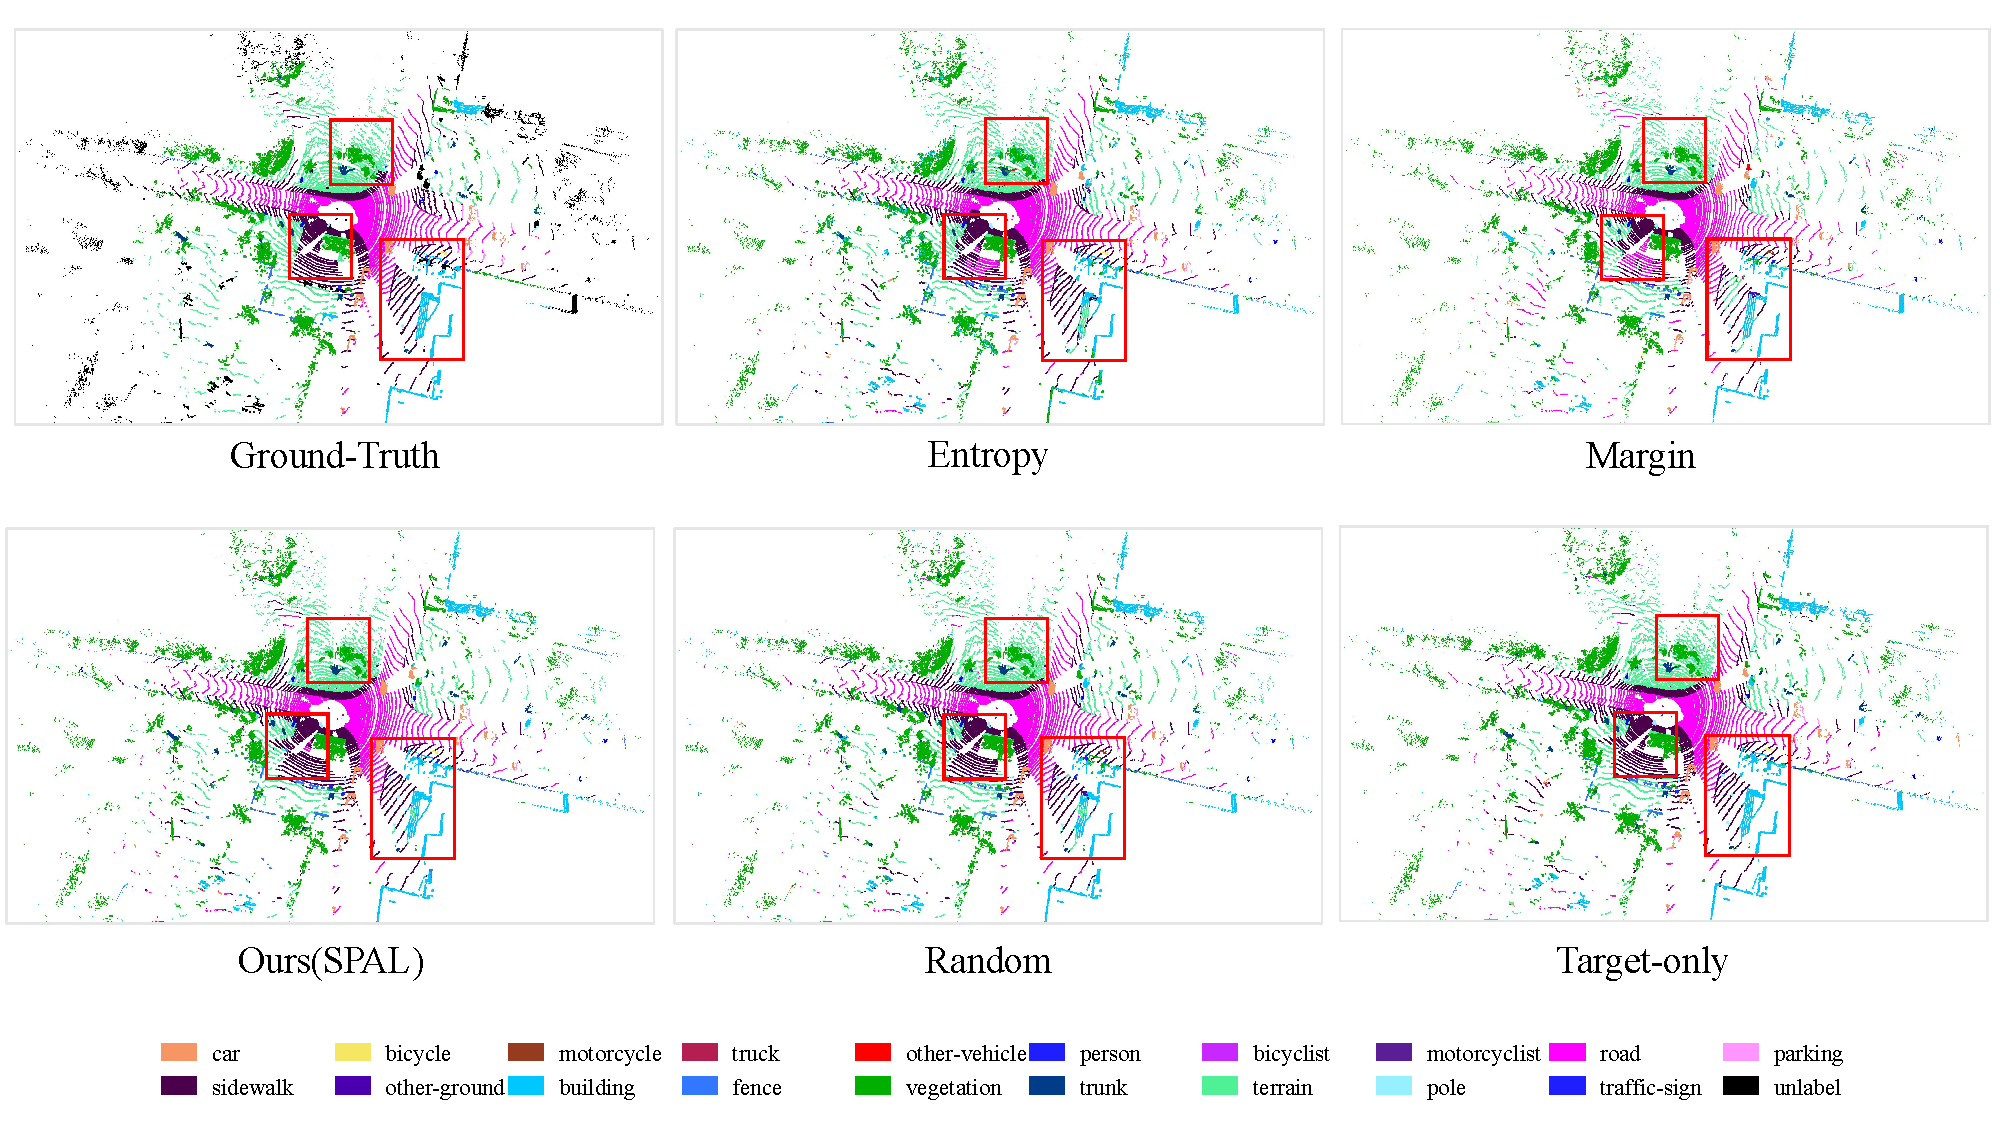
\includegraphics[width = \textwidth]{ljx/figure/3_vision_s2k1.pdf}
    \bicaption[\xiaosi 第三章SynLiDAR$\to$SemanticKITTI分割可视化图]{\wuhao 本章SynLiDAR$\to$SemanticKITTI分割可视化图}{\wuhao Visualization of the segmentation results in the SynLiDAR$\to$SemanticKITTI}
    \label{fig:3-v-1}
\end{figure}
\vspace{-0.35cm}
\vspace{0.1cm}
% \begin{table}[htbp]
\begin{table}[H]
	\renewcommand{\arraystretch}{1}
    \centering
    \setlength{\tabcolsep}{10mm}
    \bicaption[\xiaosi 第三章方法与其他域适应方法在SynLiDAR\(\to\)SemanticPOSS数据上的比较]{\wuhao 本方法与其他域适应方法在SynLiDAR\(\to\)SemanticPOSS数据上的比较}{\wuhao Comparison with other domain adaptation methods on SynLiDAR\(\to\)SemanticPOSS}
    \label{tab:3-2}
    \wuhao
    \begin{tabular}{cccc}
        \toprule[1.5pt]
        \textbf{方法} & \textbf{域适应} & \textbf{标注} & \textbf{mIoU(\%)} \\
        \midrule
        Source-Only   & -           & -       & 34.6 \\
        Target-Only   & -           & 100\%       & 58.0 \\
        % CRST          & UDA & -       & 27.1 \\
        % ST-PCT        & UDA & -       & 29.6 \\
        % PolarMix      & UDA & -       & 30.4 \\
        % CoSMix        & UDA & -       & 40.4 \\
        % DGT-ST        & UDA & -       & 50.8 \\
        CRST\upcite{zou2019confidence}          & UDA & -       & 27.1 \\
        ST-PCT\upcite{xiao2022transfer}        & UDA & -       & 29.6 \\
        PolarMix\upcite{xiao2022polarmix}      & UDA & -       & 30.4 \\
        CoSMix\upcite{saltori2022cosmix}        & UDA & -       & 40.4 \\
        DGT-ST\upcite{yuan2024density}        & UDA & -       & 50.8 \\
        % MME           & SSDA & 0.01\%  & 33.2 \\
        % APE           & SSDA & 0.01\%  & 30.3 \\
        % APE-PCT       & SSDA & 0.01\%  & 31.2 \\
        % CoSMix-SSDA   & SSDA & 0.01\%  & 41.0 \\
        % 本章方法       & SSDA   & 0.01\%   & 57.5 \\
        Annotator\upcite{Annotator}     & ADA   & 0.1\%     & 52.0 \\
        \textbf{本章方法}       & ADA   & 0.1\%     & \textbf{56.6} \\
        \bottomrule[1.5pt]
    \end{tabular}
\end{table}
实验SynLiDAR\(\to\)SemanticPOSS的结果如表\ref{tab:3-2}所示。在无监督域适应(UDA)方法中,DGT-ST仍以50.8\%的性能占据首位;
% 而在半监督域适应(SSDA)方法中,本章方法在$0.01\%$极少量标注下达到$57.5\%$逼近全监督目标域性能,同时超过CoSMix$16.5$个百分点;
而在主动域适应(ADA)方法中,本章方法在0.1\%的标注下取得56.6\%的性能超过Annotator4.6个百分点,相比全监督(Target-Only)结果仅差1.4个百分点,再一次证明了本章方法在合成到真实的跨域场景的有效性。分割可视化结果如图\ref{fig:3-v-2}所示,在红色方框所突出显示的区域中可以观察到,本章方法在一些易混淆的语义类别比如植物和建筑中的分割效果依然优于其他主动学习方法。
\begin{figure}[H]
    \centering
    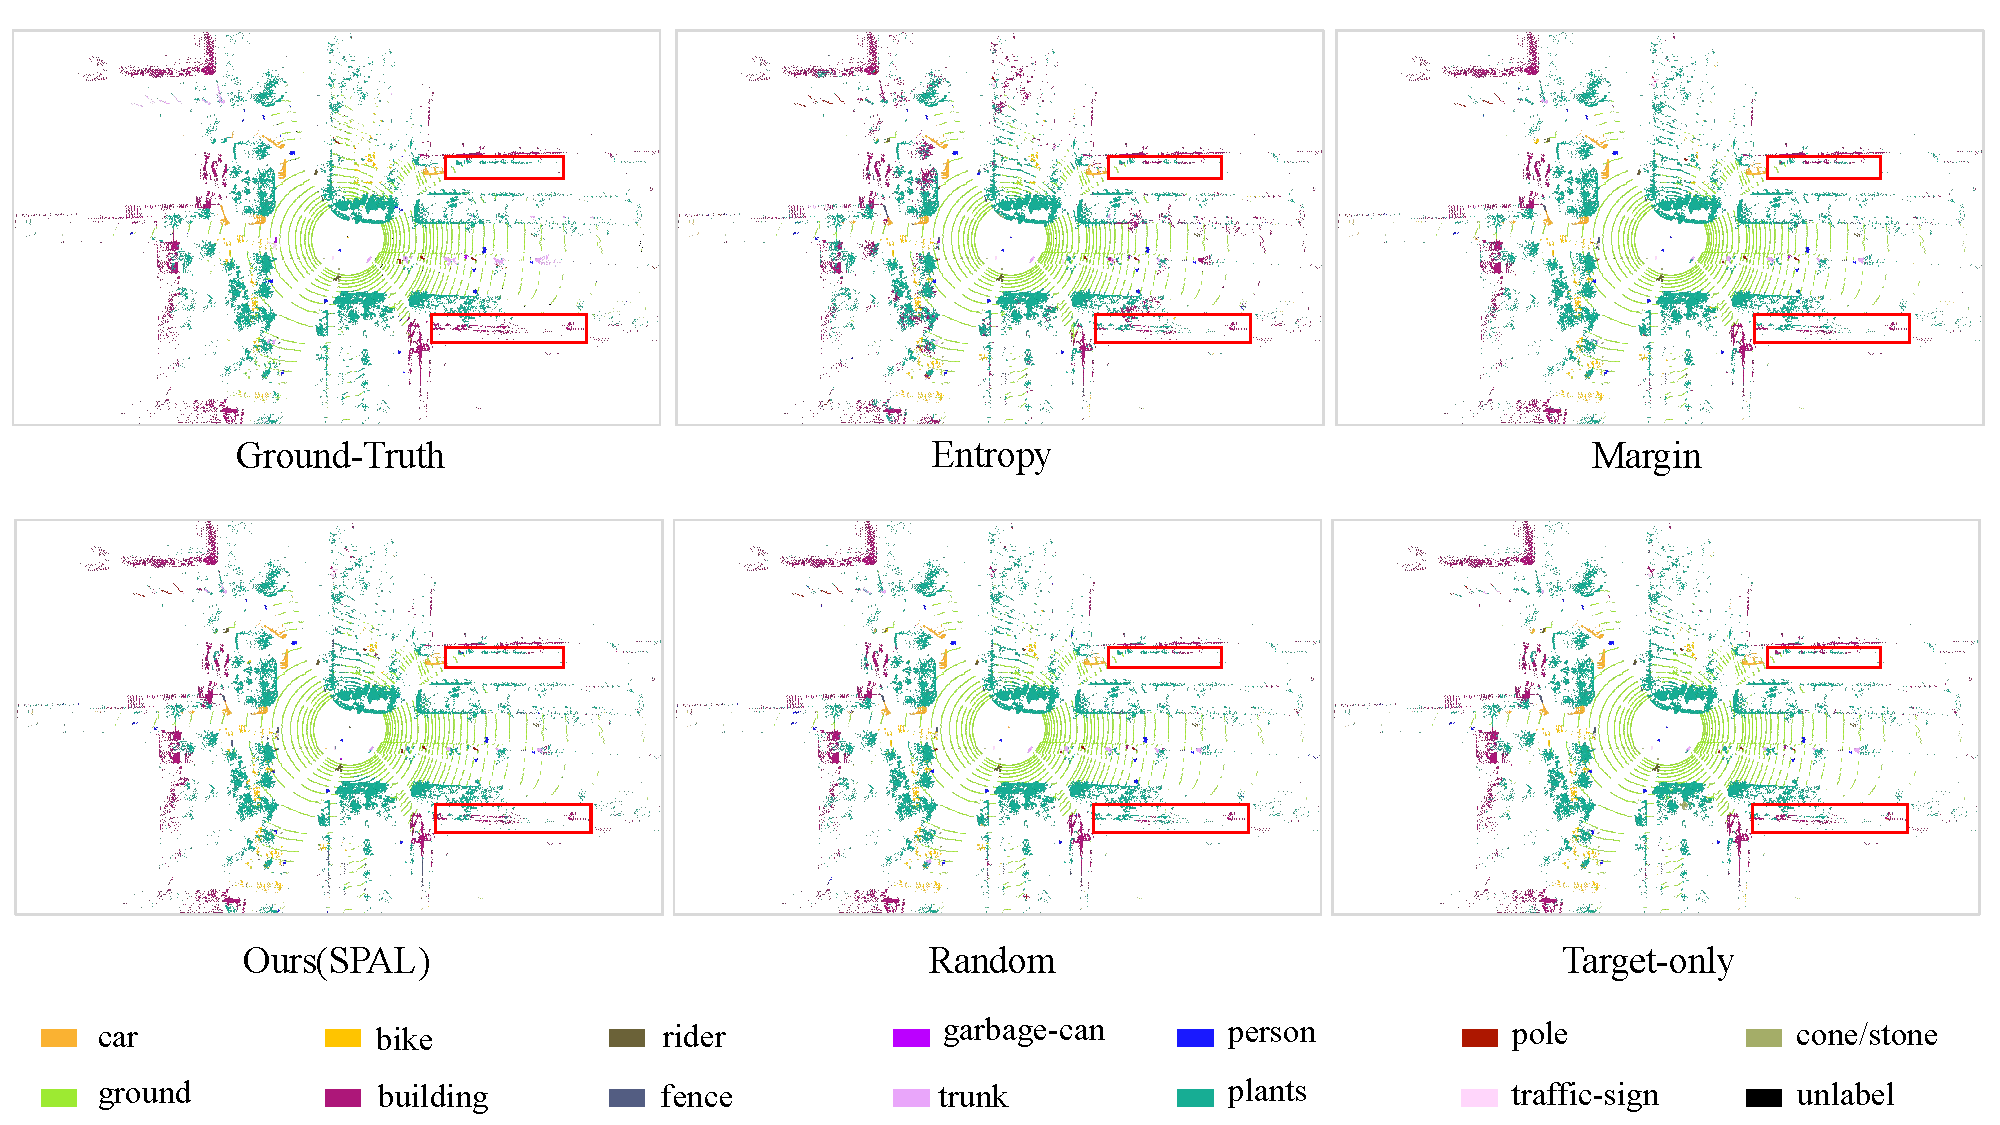
\includegraphics[width = \textwidth]{ljx/figure/3_vision_s2p.pdf}
    \bicaption[\xiaosi 第三章SynLiDAR$\to$SemanticPOSS分割可视化图]{\wuhao 本章SynLiDAR$\to$SemanticPOSS分割可视化图}{\wuhao Visualization of the segmentation results in the SynLiDAR$\to$SemanticPOSS}
    \label{fig:3-v-2}
    \vspace{-0.35cm}
\end{figure}


\subsubsection{真实到真实场景}
在合成到真实的跨域任务中,合成的数据集一般都有着标注精度更高,噪音度低的特性,因此其与真实数据集有所差异。为进一步验证方法的泛化能力,本章将方法拓展至真实到真实跨域场景,并选择nuScenes\(\to\)SemanticKITTI和SemanticKITTI\(\to\)nuScenes跨域数据集进行了实验,在此场景下,本章方法展现出与合成到真实任务相似的性能优势,进一步证明了本章方法的有效性。

如表\ref{tab:3-3}所示,在SemanticKITTI$\to$nuScenes实验中,目标域全监督基准结果与源域模型间存在49.0个百分点的性能差距,这说明在真实数据间,跨域任务要比合成更难。无监督域适应(UDA)方法中,LiDOG以34.9\%领先,但其性能仅为目标域基准的42.2\%,说明了无监督域适应在真实场景中的局限性,虽然不用进行标注但其性能仍然离全监督非常远。在主动域适应方法中(ADA),本章方法以0.1\%标注量达到目标域全监督的92.5\%,较Annotator提升0.9个百分点,验证了本章方法的有效性。同合成到真实数据集一样,本实验依然提供与Ground-Truth、Target-Only以及其他主动学习的可视化对比图。如图\ref{fig:3-v-3}所示,本章方法在一些易错类别如人行道上的分割效果依然优于其他主动学习方法,再一次验证了该方法的有效性。
% \vspace{0.1cm}
% \begin{table}[htbp]
\begin{table}[H]
	\renewcommand{\arraystretch}{1}
    \centering
    \setlength{\tabcolsep}{12mm}
    \bicaption[\xiaosi 第三章方法与其他域适应方法在SemanticKITTI\(\to\)nuScenes数据上的比较]{\wuhao 本方法与其他域适应方法在SemanticKITTI\(\to\)nuScenes数据上的比较}{\wuhao Comparison with other domain adaptation methods on SemanticKITTI\(\to\)nuScenes}
    \label{tab:3-3}
    \wuhao
    \begin{tabular}{lccc}
        \toprule[1.5pt]
        \textbf{方法} & \textbf{域适应} & \textbf{标注} & \textbf{结果} \\
        \midrule
        Source-Only   & -       & -           & 33.7 \\
        Target-Only   & -       & 100\%           & 82.7 \\
        Mix3D         & UDA     & -   & 31.5 \\
        CoSMix        & UDA     & -   & 29.8 \\
        SN              & UDA   & -     & 25.8 \\
        RayCast        & UDA    & -    & 30.9 \\
        LiDOG        & UDA      & -       & 34.9 \\
        Annotator     & ADA     & 0.1\%     & 75.9 \\
        本章方法       & ADA    & 0.1\%      & \textbf{81.0(改)} \\
        \bottomrule[1.5pt]
    \end{tabular}
\end{table}

\vspace{-0.1cm}
\begin{figure}[h]
    \centering
    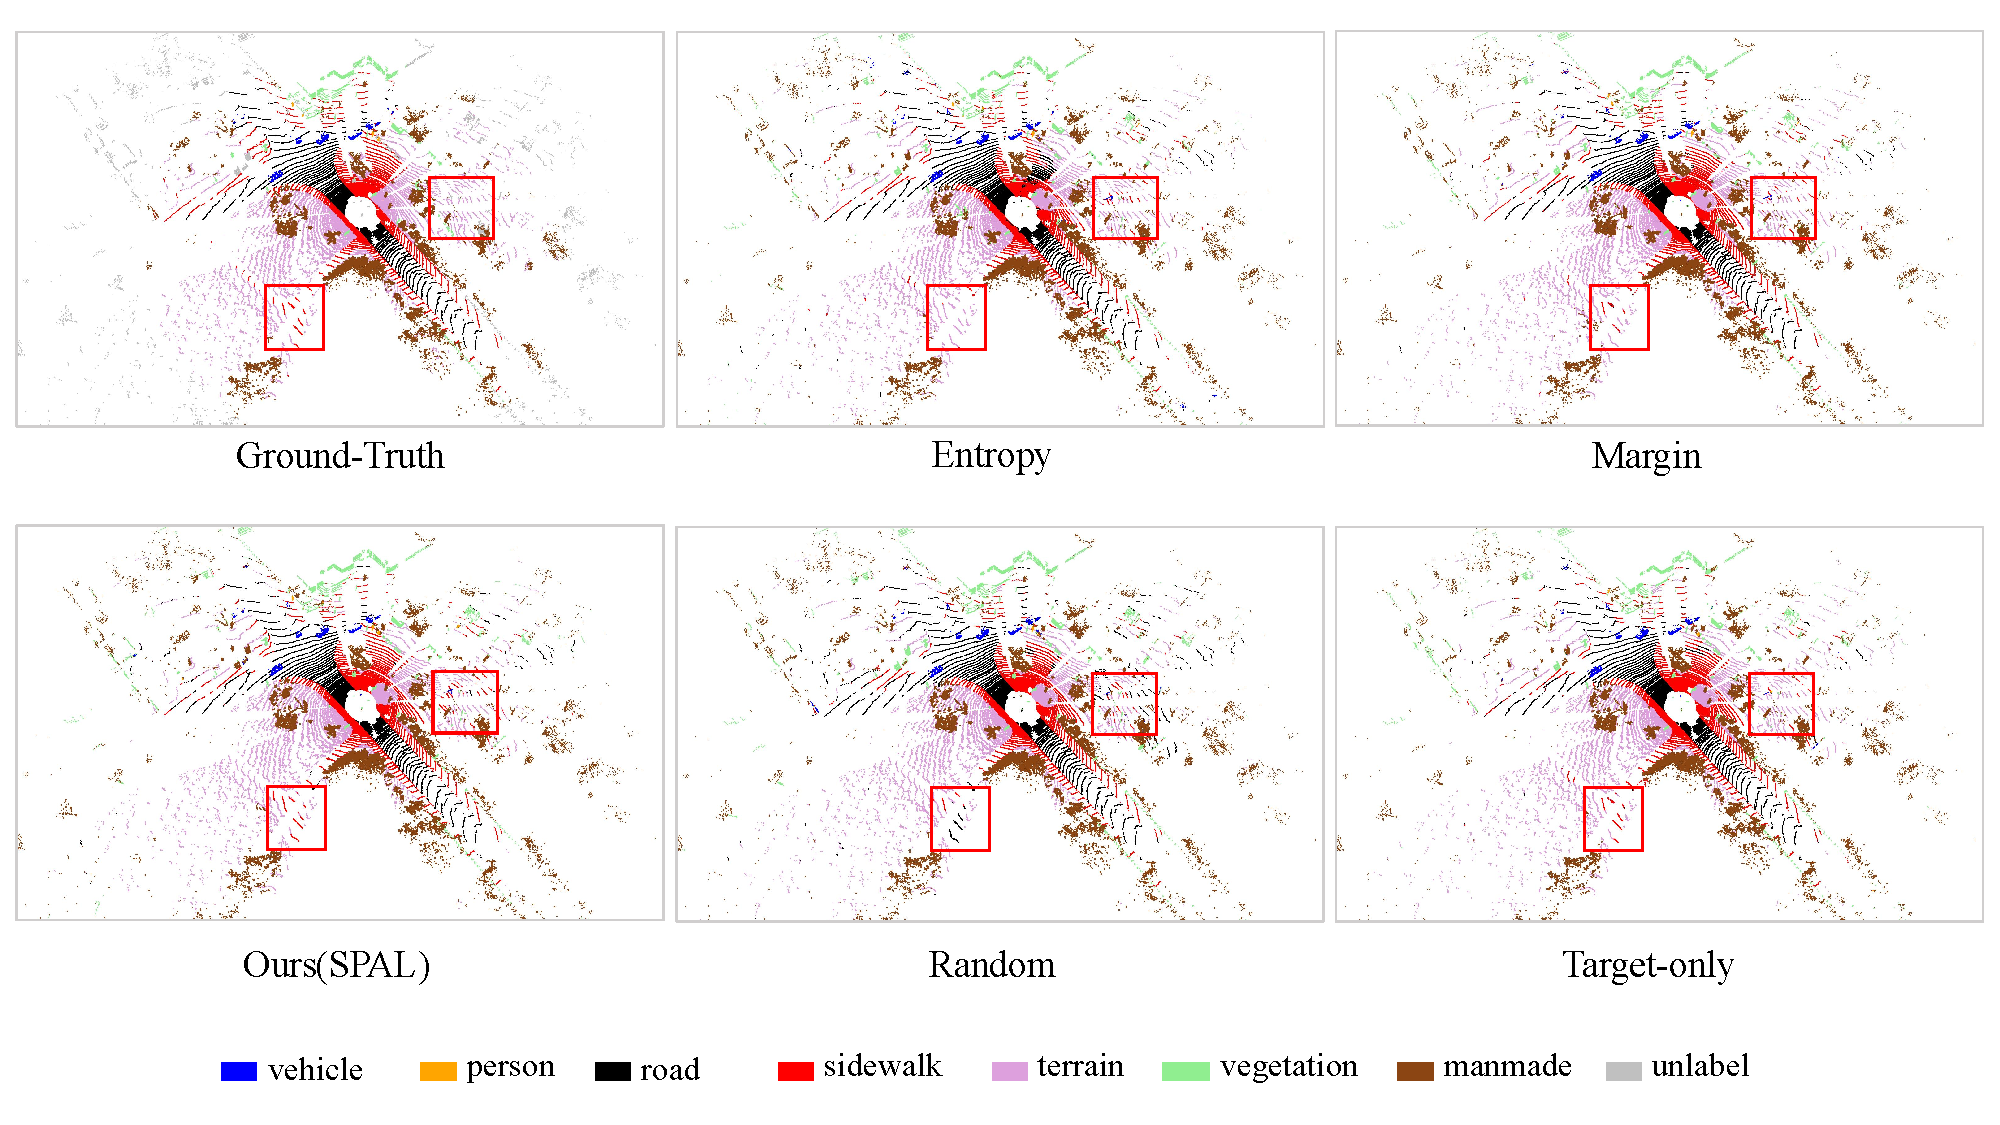
\includegraphics[width = \textwidth]{ljx/figure/3_vision_k2n.pdf}
    \bicaption[\xiaosi 第三章SemanticKITTI$\to$nuScenes分割可视化图]{\wuhao 本章SemanticKITTI$\to$nuScenes分割可视化图}{\wuhao Visualization of the segmentation results in the SemanticKITTI$\to$nuScenes}
    \label{fig:3-v-3}
\end{figure}
\vspace{-0.35cm}
在nuScenes$\to$SemanticKITTI中如表\ref{tab:3-4}所示。目标域全监督性能与源域模型性能差距进一步扩大至52.9个百分点,这说明跨域任务的难度也进一步增加。在本实验结果中,无监督域适应(UDA)最佳方法达到了41.2\%的性能,
% 比同类方法中第二高的RayCast高出9.7个百分点,
但是仍距离全监督有44.2个百分点的性能差距。值得注意的是,本章方法在0.1\%标注下取得83.0\%的结果,达到全监督性能的97\%,相较同标注量下的Annotator提升1.2个百分点。本实验也提供了分割可视化结果如图\ref{fig:3-v-4},分割证明了本章方法在此数据集上的有效性。通过实验结果可知,本章方法在真实到真实场景中均以0.1\%标注量实现超95\%全监督性能。
% 本实验相较其他主动学习、Ground-Truth、Target-Only对比的可视化结果如图\ref{fig:3-v-4}所示:
% \vspace{0.1cm}
% \begin{table}[htbp]
\begin{table}[H]
	\renewcommand{\arraystretch}{1}
    \centering
    \setlength{\tabcolsep}{12mm}
    \bicaption[\xiaosi 第三章方法与其他域适应方法在nuScenes\(\to\)SemanticKITTI数据上的比较]{\wuhao 本方法与其他域适应方法在nuScenes\(\to\)SemanticKITTI数据上的比较}{\wuhao Comparison with other domain adaptation methods on nuScenes\(\to\)SemanticKITTI}
    \label{tab:3-4}
    \wuhao
    \begin{tabular}{lccc}
        \toprule[1.5pt]
        \textbf{方法} & \textbf{域适应} & \textbf{标注} \textbf{结果} \\
        \midrule
        Target-Only   & -       & 100\%           & 85.4 \\
        Source-Only   & -       & -           & 32.5 \\
        Mix3D         & UDA     & -   & 32.4 \\
        CoSMix        & UDA     & -   & 36.8 \\
        SN              & UDA   & -     & 23.6 \\
        RayCast        & UDA    & -    & 31.5 \\
        LiDOG        & UDA      & -       & 41.2 \\
        Annotator     & ADA     & 0.1\%     & 81.8 \\
        本章方法       & ADA    & 0.1\%      & \textbf{85.4(改)} \\
        \bottomrule[1.5pt]
    \end{tabular}
\end{table}
\vspace{-0.5cm}
\begin{figure}[H]%[h]
    \centering
    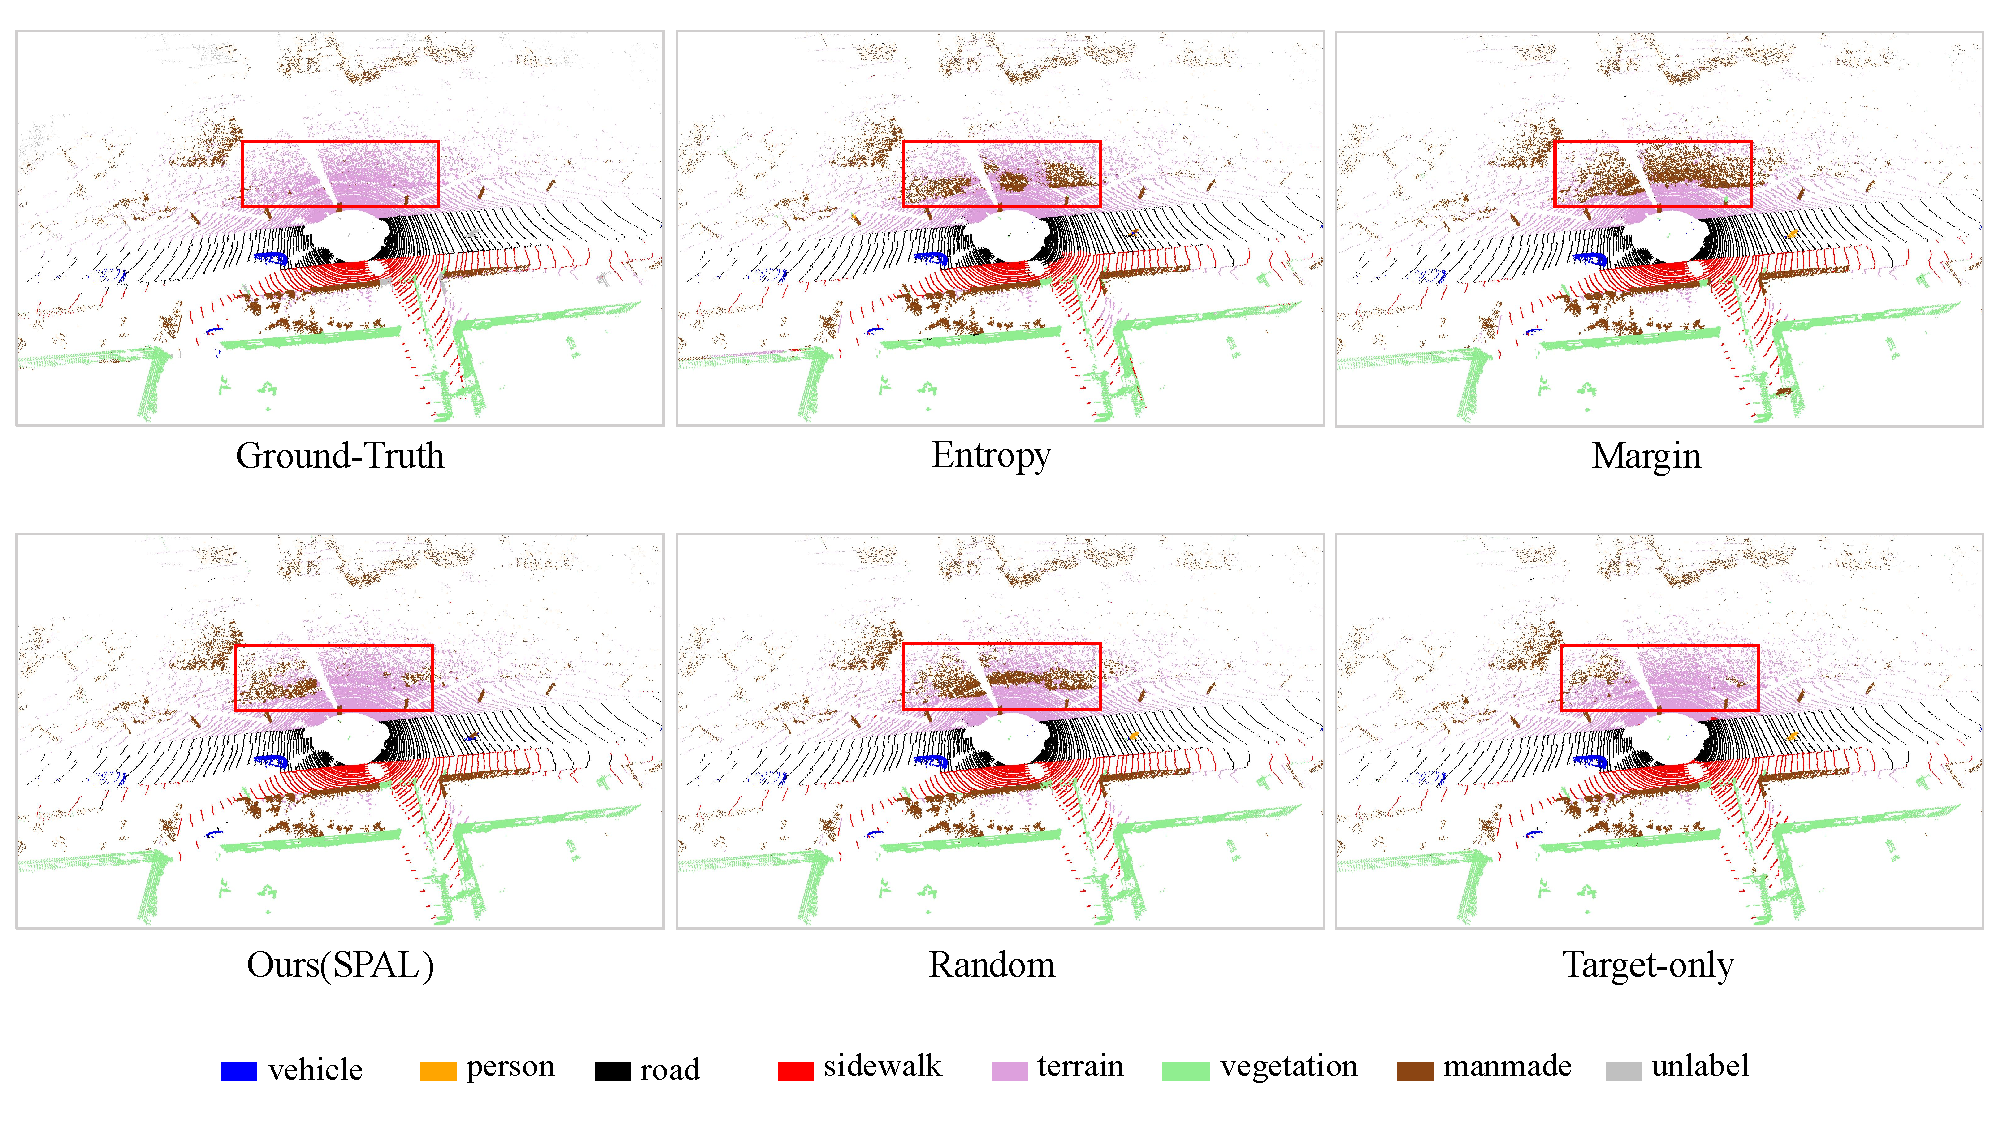
\includegraphics[width = \textwidth]{ljx/figure/3_vision_n2k.pdf}
    \bicaption[\xiaosi 第三章nuScenes$\to$SemanticKITTI分割可视化图]{\wuhao 本章nuScenes$\to$SemanticKITTI分割可视化图}{\wuhao Visualization of the segmentation results in the nuScenes$\to$SemanticKITTI}
    \label{fig:3-v-4}
\end{figure}
% \vspace{-0.35cm}
\subsection{消融对比实验}
\subsubsection{与其他主动学习方法对比}
在未引入Mixing方法时,传统主动学习方法在两类合成到真实跨域任务中表现出了一定的优势如表\ref{tab:3-5}所示。在SynLiDAR$\to$SemanticKITTI任务中,Margin方法以54.4\%的性能取得最优结果,而本章主动学习方法SPAL以53.5\%略低1.1个百分点,但仍然超过了Random0.2个百分点Entropy2.8个百分点。究其原因,本章的方法是通过源域而构建起的原型,比较依赖源域信息,在没有Mixing混合源数据的情况下,构建的原型就不可靠,因此无法发挥最大的效果。
而在SynLiDAR$\to$SemanticPOSS任务中,
% 本章的主动学习策略(SPAL)
SPAL低于Entropy 0.7个百分点,却也超过了Random 3.2个百分点,Margin 0.2个百分点,这一结果表明,传统主动学习策略在特定场景下仍具竞争力,但单一采样准则难以适应跨域任务的复杂性。

\vspace{0.1cm}
% \begin{table}[htbp]
\begin{table}[H]
	\renewcommand{\arraystretch}{1}
    \centering
    \setlength{\tabcolsep}{10mm}
    \bicaption[\xiaosi 第三章主动学习方法与其他传统主动学习方法对比]{\wuhao 本章的主动学习方法与其他传统主动学习方法对比}{\wuhao  Comparison with other active learning methods}
    \label{tab:3-5}
    \wuhao
    \begin{tabular}{cccc}
        \toprule[1.5pt]
        \textbf{数据集} & \textbf{方法} & \textbf{标注} & \textbf{结果} \\
        \midrule
        \multirow{4}{*}{SynLiDAR\(\to\)SemanticKITTI} & 
        Random              & 0.1\%        & 53.2 \\
        ~ & Entropy\upcite{Entropy}             & 0.1\%        & 51.7 \\
        ~ & \textbf{Margin}\upcite{Margin}              & 0.1\%        & \textbf{54.4} \\
        ~ & Ours(SPAL)          & 0.1\%        & 53.5 \\
        \multirow{4}{*}{SynLiDAR\(\to\)SemanticPOSS} & 
        Random              & 0.1\%        & 47.5 \\
        ~ & \textbf{Entropy}\upcite{Entropy}             & 0.1\%        & \textbf{51.4} \\
        ~ & Margin\upcite{Margin}              & 0.1\%        & 50.5 \\
        ~ & Ours(SPAL)          & 0.1\%        & 50.7 \\
        \bottomrule[1.5pt]
    \end{tabular}
\end{table}

而在结合Mixing方法后如表\ref{tab:3-6}所示,除Random以外各主动学习方法在SynLiDAR$\to$SemanticKITTI任务中的性能均显著提升,其中本章主动学习方法SPAL以58.7\%的性能达到最优,较次优的Margin方法提升1.1个百分点,较未结合Mixing时的自身结果提升5.2个百分点,Margin、Entropy则分别较自身提升3.2和3.4个百分点。这表明结合主动学习和Mixing策略的有效性,通过主动筛选出的标注目标点和源点动态构建中间域数据可以有效提升模型的性能,进一步缓解域间分布差异。但Random方法下降了2.1个百分点,这说明性能增益也与主动学习方法有关系,混合中间域信息包含域差异信息越丰富,其提升程度越高,而本章方法选择的是域差异性和不确定性最高的点,因此提升幅度最大。而在SynLiDAR$\to$SemanticPOSS任务中,Random、Entropy、Margin和SPAL分别提升4.4、1、5.2和5.9个百分点,
% 各主动学习方法结合Mixing后均有所提升,
进一步证明了主动学习和Mixing策略结合的有效性。
\vspace{0.1cm}
% \begin{table}[htbp]
\begin{table}[H]
	\renewcommand{\arraystretch}{1}
    \centering
    \setlength{\tabcolsep}{10mm}
    \bicaption[\xiaosi 第三章主动学习方法与其他传统主动学习方法在结合Mixing后的对比]{\wuhao 本章主动学习方法与其他传统主动学习方法在结合Mixing后的对比}{\wuhao  Comparison with other active learning methods after integrating Mixing}
    \label{tab:3-6}
    \wuhao
    \begin{tabular}{cccc}
        \toprule[1.5pt]
        \textbf{数据集} & \textbf{方法} & \textbf{标注} & \textbf{结果} \\
        \midrule
        \multirow{4}{*}{SynLiDAR\(\to\)SemanticKITTI}
        & Random              & 0.1\%        & 51.1 \\
        ~ & Entropy\upcite{Entropy}             & 0.1\%        & 55.1 \\
        ~ & Margin\upcite{Margin}              & 0.1\%        & 57.6 \\
        ~ & \textbf{Ours(SPAL)}          & 0.1\%        & \textbf{58.7} \\
        \bottomrule[1.5pt]
    \end{tabular}
\end{table}

\subsubsection{消融实验}
为证明方法的有效性,本章在SynLiDAR$\to$SemanticKITTI数据上进行了消融实验,默认使用0.1\%的标注,结果如表\ref{tab:3-7}所示,本章提出的源域指导的主动学习方法SPAL与Mixing方法构建的中间域数据对模型性能具有显著协同优化作用。仅使用Mixing,模型性能为51.2\%,较无任何模块的基线提升28.3个百分点,验证了跨域数据融合对缓解域间分布差异的有效性。而当仅使用SPAL时,模型性能提升至53.5\%,较基线增加30.7个百分点,证明了原型指导的数据选择主动学习方法对目标域关键样本筛选的优势。而当二者联合使用时,模型以58.7\%的结果达到最优,较单一模块性能分别提升7.5和5.2个百分点,表明本章方法的真实有效性。
\vspace{0.1cm}
% \begin{table}[htbp]
% 	\renewcommand{\arraystretch}{1}
%     \centering
%     \setlength{\tabcolsep}{2mm}
%     \bicaption[\xiaosi 第三章方法与先进方法关于内点率的比较]{\wuhao 本方法与先进方法关于内点率的比较}{\wuhao Comparison of Inlier Ratio between this method and advanced methods}
%     \label{tab:3-7}
%     \wuhao
%     \begin{tabular}{lccc}
%         \toprule[1.5pt]
%         \textbf{方法} & \textbf{主动学习(SPAL)} & \textbf{Mixing} & \textbf{结果} \\
%         \midrule
%         \multirow{4}{*}{SynLiDAR\(\to\)SemanticKITTI} &
%           &            &           22.8\\
%         ~ &      \checkmark &         & 50.7 \\
%         ~ &              &  \checkmark        & running... \\
%         ~ & \checkmark          & \checkmark        & \textbf{58.7} \\
%         \bottomrule[1.5pt]
%     \end{tabular}
% \end{table}

% \begin{table}[htbp]
\begin{table}[H]
	\renewcommand{\arraystretch}{1}
    \centering
    \setlength{\tabcolsep}{10mm}
    \bicaption[\xiaosi 第三章方法消融实验]{\wuhao 本章方法模块消融实验}{\wuhao Ablation experiments on modules}
    \label{tab:3-7}
    \wuhao
    \begin{tabular}{ccc}
        \toprule[1.5pt]
        \textbf{主动学习(SPAL)} & \textbf{Mixing} & \textbf{结果} \\
        \midrule
          &             &                   22.8\\
        \checkmark      &               &   50.7 \\
                        &  \checkmark        & 51.2 \\
         \checkmark          & \checkmark        & \textbf{58.7} \\
        \bottomrule[1.5pt]
    \end{tabular}
\end{table}

\section{本章小结}
本章主要研究适用于点云语义分割域适应任务的主动学习方法。为了解决传统主动学习方法中的不足,提出了一种原型指导的主动学习策略,该策略通过动态构建源域原型来代表源域类别质心,并在每一轮主动学习阶段实时更新原型,在进行目标域候选点筛选时,计算每个目标域中未标注的点与每个源域类别原型的相似度,通过最优-次优差异算法获取归一化后的类别概率的差值得到域差异性评分,值越小说明该点域差异性越高,同时结合不确定性评分得到最终候选评分,升序排列后选取前k个同时兼备高不确定性和高域差异性的目标点。此外,本章首次将主动学习方法与Mixing方法结合并用于点云语义分割域适应任务中,构建包含目标域信息和源域信息的中间域数据,帮助模型学习到更稳定的域不变特征,进一步缩小域间隙。在本章中,首先介绍了方法的主要框架和流程,并分别对方法中的三个模块做了详细介绍,这三个模块共同组成了本章的方法,大幅度提升了模型的跨域性能。同时, 为了验证方法的有效性,在两个跨域场景四个数据集上进行了大量实验,并与此前最有效的点云语义分割无监督域适应和主动域适应进行了对比,通过实验分析验证了本章方法的有效性,最后进一步对Mixing和SPAL模块进行消融实验,充分验证了两个模块的有效性。

% 验证AL与mix的有效性
% 验证不同参数下的结果
% 验证不同预算下的结果